% Jerarquia simplicial: paso de mensajes multi-orden
% Compilar con: pdflatex simplicial_hierarchy.tex
\documentclass[tikz,border=10pt]{standalone}
\usepackage{tikz}
\usepackage{amsmath,amssymb}

\definecolor{gdlblue}{RGB}{41, 98, 168}
\definecolor{gdlred}{RGB}{191, 49, 49}
\definecolor{gdlgreen}{RGB}{30, 130, 76}
\definecolor{gdlorange}{RGB}{217, 130, 30}
\definecolor{gdlpurple}{RGB}{118, 56, 138}
\definecolor{gdlgray}{RGB}{140, 140, 140}
\definecolor{gdlyellow}{RGB}{190, 140, 10}

\usetikzlibrary{arrows.meta, positioning, calc, backgrounds}

\begin{document}
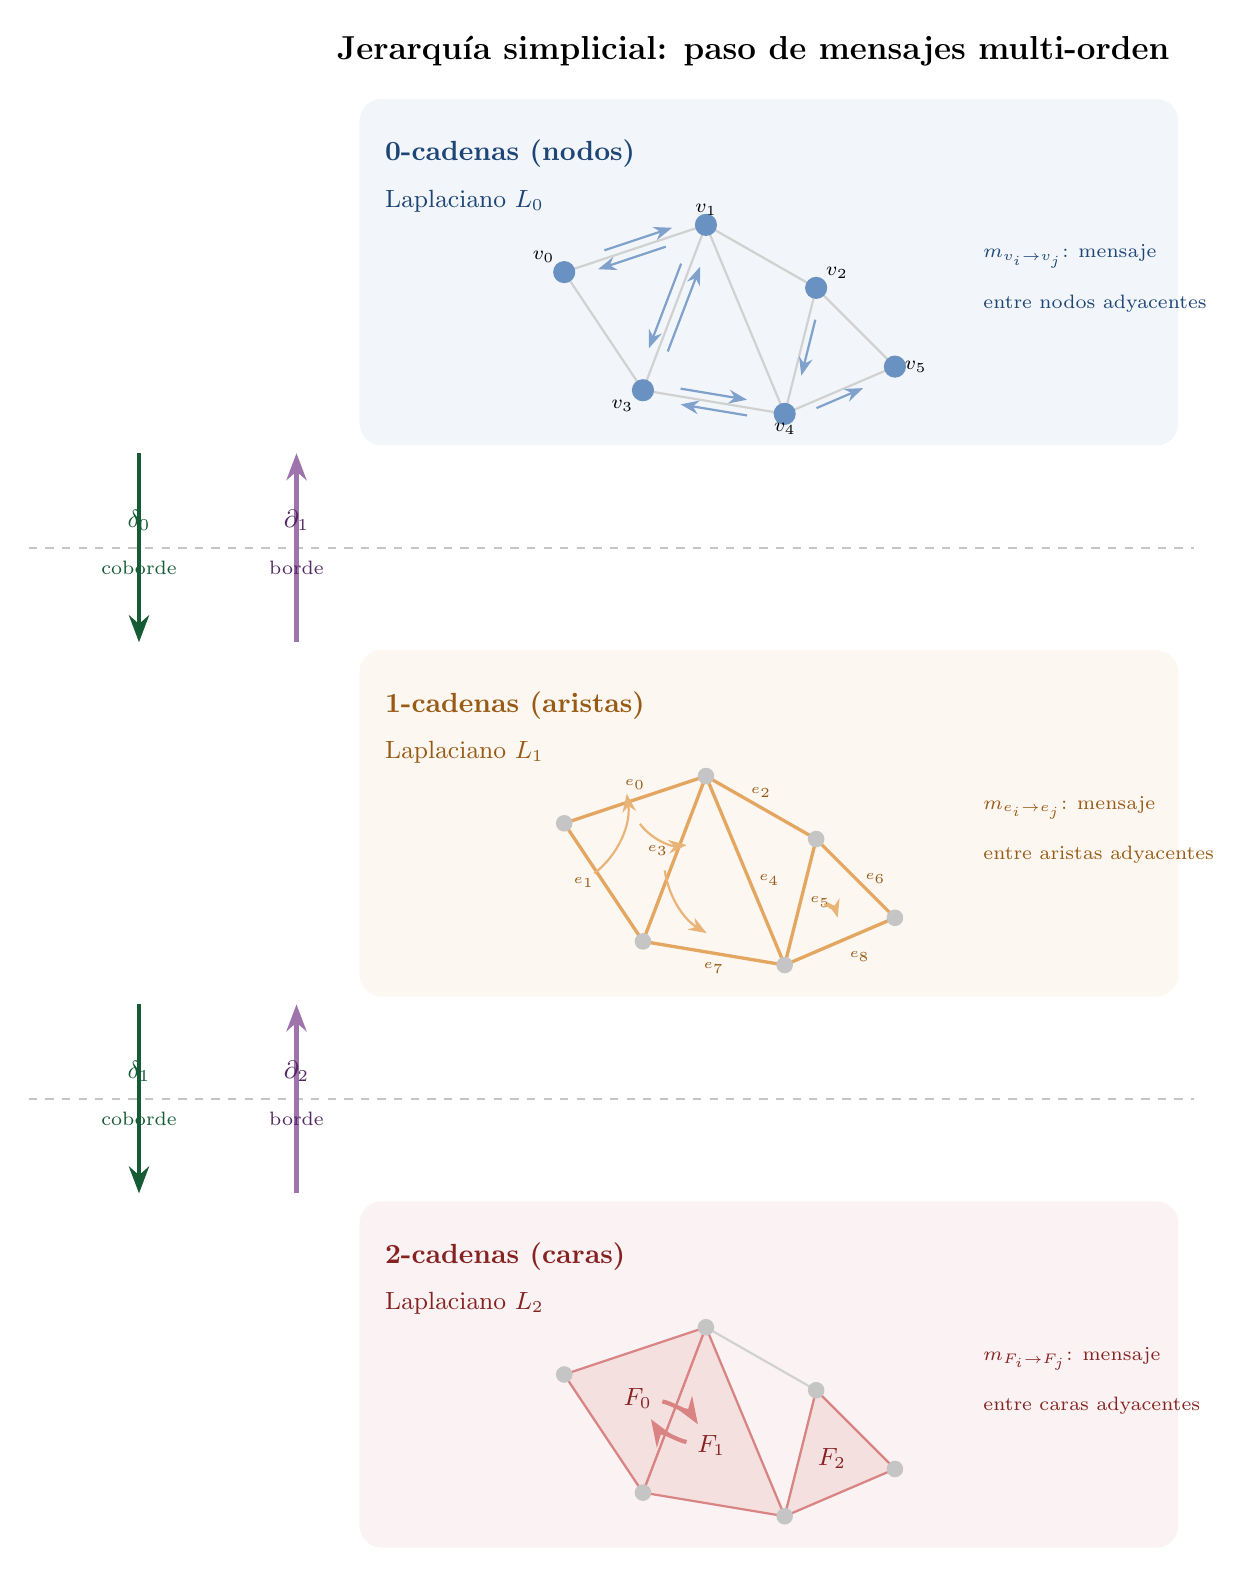
\begin{tikzpicture}[>=Stealth, font=\small]

% ============================================================
% Vertical offsets for the three levels
% ============================================================
\def\leveltop{7}
\def\levelmid{0}
\def\levelbot{-7}

% ============================================================
% Background shading for each level (drawn first)
% ============================================================
\begin{scope}[on background layer]
    \fill[gdlblue!6, rounded corners=8pt]
        (-2.6, \leveltop-2.2) rectangle (7.8, \leveltop+2.2);
    \fill[gdlorange!6, rounded corners=8pt]
        (-2.6, \levelmid-2.2) rectangle (7.8, \levelmid+2.2);
    \fill[gdlred!6, rounded corners=8pt]
        (-2.6, \levelbot-2.2) rectangle (7.8, \levelbot+2.2);
\end{scope}

% Separators between levels
\draw[dashed, gdlgray!50, line width=0.8pt]
    (-6.8, {(\leveltop+\levelmid)/2}) -- (8, {(\leveltop+\levelmid)/2});
\draw[dashed, gdlgray!50, line width=0.8pt]
    (-6.8, {(\levelmid+\levelbot)/2}) -- (8, {(\levelmid+\levelbot)/2});

% Title
\node[font=\bfseries\large, text=black] at (2.4, \leveltop+2.8)
    {Jerarqu\'ia simplicial: paso de mensajes multi-orden};

% ============================================================
% LEVEL 0: 0-chains (nodes) -- message passing between nodes
% ============================================================
\begin{scope}[shift={(0, \leveltop)}]

    % Level label
    \node[font=\bfseries, text=gdlblue!70!black, anchor=west] at (-2.4, 1.5)
        {0-cadenas (nodos)};
    \node[font=\small, text=gdlblue!70!black, anchor=west] at (-2.4, 0.9)
        {Laplaciano $L_0$};

    % Edges (background, subdued)
    \draw[gdlgray!40, thick] (0,0) -- (1.8,0.6);
    \draw[gdlgray!40, thick] (0,0) -- (1.0,-1.5);
    \draw[gdlgray!40, thick] (1.8,0.6) -- (3.2,-0.2);
    \draw[gdlgray!40, thick] (1.8,0.6) -- (1.0,-1.5);
    \draw[gdlgray!40, thick] (1.8,0.6) -- (2.8,-1.8);
    \draw[gdlgray!40, thick] (3.2,-0.2) -- (2.8,-1.8);
    \draw[gdlgray!40, thick] (3.2,-0.2) -- (4.2,-1.2);
    \draw[gdlgray!40, thick] (1.0,-1.5) -- (2.8,-1.8);
    \draw[gdlgray!40, thick] (2.8,-1.8) -- (4.2,-1.2);

    % Message arrows between adjacent nodes (selected pairs)
    % v0 -> v1
    \draw[->, gdlblue!60, thick, shorten >=6pt, shorten <=6pt]
        ($(0,0)!0.15!(1.8,0.6)+(0.04, 0.12)$) -- ($(0,0)!0.85!(1.8,0.6)+(0.04,0.12)$);
    % v1 -> v0
    \draw[->, gdlblue!60, thick, shorten >=6pt, shorten <=6pt]
        ($(1.8,0.6)!0.15!(0,0)+(-0.04,-0.12)$) -- ($(1.8,0.6)!0.85!(0,0)+(-0.04,-0.12)$);
    % v1 -> v3
    \draw[->, gdlblue!60, thick, shorten >=6pt, shorten <=6pt]
        ($(1.8,0.6)!0.15!(1.0,-1.5)+(-0.12, 0.02)$) -- ($(1.8,0.6)!0.85!(1.0,-1.5)+(-0.12, 0.02)$);
    % v3 -> v1
    \draw[->, gdlblue!60, thick, shorten >=6pt, shorten <=6pt]
        ($(1.0,-1.5)!0.15!(1.8,0.6)+(0.12, -0.02)$) -- ($(1.0,-1.5)!0.85!(1.8,0.6)+(0.12, -0.02)$);
    % v3 -> v4
    \draw[->, gdlblue!60, thick, shorten >=6pt, shorten <=6pt]
        ($(1.0,-1.5)!0.15!(2.8,-1.8)+(0, 0.1)$) -- ($(1.0,-1.5)!0.85!(2.8,-1.8)+(0, 0.1)$);
    % v4 -> v3
    \draw[->, gdlblue!60, thick, shorten >=6pt, shorten <=6pt]
        ($(2.8,-1.8)!0.15!(1.0,-1.5)+(0,-0.1)$) -- ($(2.8,-1.8)!0.85!(1.0,-1.5)+(0,-0.1)$);
    % v2 -> v4
    \draw[->, gdlblue!60, thick, shorten >=6pt, shorten <=6pt]
        ($(3.2,-0.2)!0.15!(2.8,-1.8)+(0.1, 0.04)$) -- ($(3.2,-0.2)!0.85!(2.8,-1.8)+(0.1,0.04)$);
    % v4 -> v5
    \draw[->, gdlblue!60, thick, shorten >=6pt, shorten <=6pt]
        ($(2.8,-1.8)!0.15!(4.2,-1.2)+(0, -0.1)$) -- ($(2.8,-1.8)!0.85!(4.2,-1.2)+(0,-0.1)$);

    % Nodes (on top)
    \fill[gdlblue!70] (0,0) circle (4pt);
    \fill[gdlblue!70] (1.8,0.6) circle (4pt);
    \fill[gdlblue!70] (3.2,-0.2) circle (4pt);
    \fill[gdlblue!70] (1.0,-1.5) circle (4pt);
    \fill[gdlblue!70] (2.8,-1.8) circle (4pt);
    \fill[gdlblue!70] (4.2,-1.2) circle (4pt);

    % Node labels
    \node[above left, font=\scriptsize] at (0,0) {$v_0$};
    \node[above, font=\scriptsize] at (1.8,0.6) {$v_1$};
    \node[above right, font=\scriptsize] at (3.2,-0.2) {$v_2$};
    \node[below left, font=\scriptsize] at (1.0,-1.5) {$v_3$};
    \node[below, font=\scriptsize] at (2.8,-1.8) {$v_4$};
    \node[right, font=\scriptsize] at (4.2,-1.2) {$v_5$};

    % Legend annotation
    \node[font=\scriptsize, text=gdlblue!70!black, anchor=west] at (5.2, 0.2)
        {$m_{v_i \to v_j}$: mensaje};
    \node[font=\scriptsize, text=gdlblue!70!black, anchor=west] at (5.2, -0.4)
        {entre nodos adyacentes};
\end{scope}

% ============================================================
% LEVEL 1: 1-chains (edges) -- message passing between edges
% ============================================================
\begin{scope}[shift={(0, \levelmid)}]

    % Level label
    \node[font=\bfseries, text=gdlorange!70!black, anchor=west] at (-2.4, 1.5)
        {1-cadenas (aristas)};
    \node[font=\small, text=gdlorange!70!black, anchor=west] at (-2.4, 0.9)
        {Laplaciano $L_1$};

    % Edges as thick orange lines (primary objects at this level)
    \draw[gdlorange!70, very thick] (0,0) -- (1.8,0.6);          % e0
    \draw[gdlorange!70, very thick] (0,0) -- (1.0,-1.5);         % e1
    \draw[gdlorange!70, very thick] (1.8,0.6) -- (3.2,-0.2);    % e2
    \draw[gdlorange!70, very thick] (1.8,0.6) -- (1.0,-1.5);    % e3
    \draw[gdlorange!70, very thick] (1.8,0.6) -- (2.8,-1.8);    % e4
    \draw[gdlorange!70, very thick] (3.2,-0.2) -- (2.8,-1.8);   % e5
    \draw[gdlorange!70, very thick] (3.2,-0.2) -- (4.2,-1.2);   % e6
    \draw[gdlorange!70, very thick] (1.0,-1.5) -- (2.8,-1.8);   % e7
    \draw[gdlorange!70, very thick] (2.8,-1.8) -- (4.2,-1.2);   % e8

    % Nodes (subdued, on top of edges)
    \fill[gdlgray!50] (0,0) circle (3pt);
    \fill[gdlgray!50] (1.8,0.6) circle (3pt);
    \fill[gdlgray!50] (3.2,-0.2) circle (3pt);
    \fill[gdlgray!50] (1.0,-1.5) circle (3pt);
    \fill[gdlgray!50] (2.8,-1.8) circle (3pt);
    \fill[gdlgray!50] (4.2,-1.2) circle (3pt);

    % Edge labels (midpoints)
    \node[above, font=\tiny, text=gdlorange!70!black]
        at ($(0,0)!0.5!(1.8,0.6)$) {$e_0$};
    \node[left, font=\tiny, text=gdlorange!70!black]
        at ($(0,0)!0.5!(1.0,-1.5)$) {$e_1$};
    \node[above, font=\tiny, text=gdlorange!70!black]
        at ($(1.8,0.6)!0.5!(3.2,-0.2)$) {$e_2$};
    \node[left, font=\tiny, text=gdlorange!70!black]
        at ($(1.8,0.6)!0.45!(1.0,-1.5)$) {$e_3$};
    \node[right, font=\tiny, text=gdlorange!70!black]
        at ($(1.8,0.6)!0.55!(2.8,-1.8)$) {$e_4$};
    \node[right, font=\tiny, text=gdlorange!70!black]
        at ($(3.2,-0.2)!0.5!(2.8,-1.8)$) {$e_5$};
    \node[right, font=\tiny, text=gdlorange!70!black]
        at ($(3.2,-0.2)!0.5!(4.2,-1.2)$) {$e_6$};
    \node[below, font=\tiny, text=gdlorange!70!black]
        at ($(1.0,-1.5)!0.5!(2.8,-1.8)$) {$e_7$};
    \node[below right, font=\tiny, text=gdlorange!70!black]
        at ($(2.8,-1.8)!0.5!(4.2,-1.2)$) {$e_8$};

    % Messages between adjacent edges (edges sharing a vertex)
    % e0 -> e3 (share v1): curved arrow between midpoints
    \draw[->, gdlorange!60, thick, shorten >=3pt, shorten <=3pt]
        ($(0,0)!0.5!(1.8,0.6)+(0,-0.22)$) to[bend right=30]
        ($(1.8,0.6)!0.45!(1.0,-1.5)+(0.22,0.08)$);
    % e3 -> e7 (share v3): curved arrow
    \draw[->, gdlorange!60, thick, shorten >=3pt, shorten <=3pt]
        ($(1.8,0.6)!0.45!(1.0,-1.5)+(-0.18,-0.15)$) to[bend right=25]
        ($(1.0,-1.5)!0.5!(2.8,-1.8)+(0,0.2)$);
    % e5 -> e8 (share v4): curved arrow
    \draw[->, gdlorange!60, thick, shorten >=3pt, shorten <=3pt]
        ($(3.2,-0.2)!0.5!(2.8,-1.8)+(0.2,0)$) to[bend left=30]
        ($(2.8,-1.8)!0.5!(4.2,-1.2)+(0,0.2)$);
    % e1 -> e0 (share v0): curved arrow
    \draw[->, gdlorange!60, thick, shorten >=3pt, shorten <=3pt]
        ($(0,0)!0.5!(1.0,-1.5)+(-0.2,0.05)$) to[bend right=30]
        ($(0,0)!0.5!(1.8,0.6)+(-0.12,0.18)$);

    % Legend annotation
    \node[font=\scriptsize, text=gdlorange!70!black, anchor=west] at (5.2, 0.2)
        {$m_{e_i \to e_j}$: mensaje};
    \node[font=\scriptsize, text=gdlorange!70!black, anchor=west] at (5.2, -0.4)
        {entre aristas adyacentes};
\end{scope}

% ============================================================
% LEVEL 2: 2-chains (faces) -- message passing between faces
% ============================================================
\begin{scope}[shift={(0, \levelbot)}]

    % Level label
    \node[font=\bfseries, text=gdlred!70!black, anchor=west] at (-2.4, 1.5)
        {2-cadenas (caras)};
    \node[font=\small, text=gdlred!70!black, anchor=west] at (-2.4, 0.9)
        {Laplaciano $L_2$};

    % Non-face edges first (behind faces)
    \draw[gdlgray!40, thick] (0,0) -- (1.0,-1.5);
    \draw[gdlgray!40, thick] (1.8,0.6) -- (3.2,-0.2);
    \draw[gdlgray!40, thick] (1.8,0.6) -- (2.8,-1.8);
    \draw[gdlgray!40, thick] (3.2,-0.2) -- (2.8,-1.8);
    \draw[gdlgray!40, thick] (3.2,-0.2) -- (4.2,-1.2);
    \draw[gdlgray!40, thick] (2.8,-1.8) -- (4.2,-1.2);

    % Filled triangular faces
    % Face F0: (v0, v1, v3)
    \fill[gdlred!15] (0,0) -- (1.8,0.6) -- (1.0,-1.5) -- cycle;
    \draw[gdlred!60, thick] (0,0) -- (1.8,0.6) -- (1.0,-1.5) -- cycle;

    % Face F1: (v1, v3, v4)
    \fill[gdlred!15] (1.8,0.6) -- (1.0,-1.5) -- (2.8,-1.8) -- cycle;
    \draw[gdlred!60, thick] (1.8,0.6) -- (1.0,-1.5) -- (2.8,-1.8) -- cycle;

    % Face F2: (v2, v4, v5)
    \fill[gdlred!15] (3.2,-0.2) -- (2.8,-1.8) -- (4.2,-1.2) -- cycle;
    \draw[gdlred!60, thick] (3.2,-0.2) -- (2.8,-1.8) -- (4.2,-1.2) -- cycle;

    % Nodes (subdued, on top)
    \fill[gdlgray!50] (0,0) circle (3pt);
    \fill[gdlgray!50] (1.8,0.6) circle (3pt);
    \fill[gdlgray!50] (3.2,-0.2) circle (3pt);
    \fill[gdlgray!50] (1.0,-1.5) circle (3pt);
    \fill[gdlgray!50] (2.8,-1.8) circle (3pt);
    \fill[gdlgray!50] (4.2,-1.2) circle (3pt);

    % Face labels at centroids
    % F0: centroid = (0.933, -0.3)
    \node[font=\small\bfseries, text=gdlred!70!black] at (0.933, -0.3) {$F_0$};
    % F1: centroid = (1.867, -0.9)
    \node[font=\small\bfseries, text=gdlred!70!black] at (1.867, -0.9) {$F_1$};
    % F2: centroid = (3.4, -1.067)
    \node[font=\small\bfseries, text=gdlred!70!black] at (3.4, -1.067) {$F_2$};

    % Messages between adjacent faces (faces sharing an edge)
    % F0 <-> F1 share edge (v1,v3): bidirectional curved arrows
    \draw[->, gdlred!60, line width=1.5pt, shorten >=9pt, shorten <=9pt]
        (0.933, -0.3) to[bend left=25] (1.867, -0.9);
    \draw[->, gdlred!60, line width=1.5pt, shorten >=9pt, shorten <=9pt]
        (1.867, -0.9) to[bend left=25] (0.933, -0.3);

    % Legend annotation
    \node[font=\scriptsize, text=gdlred!70!black, anchor=west] at (5.2, 0.2)
        {$m_{F_i \to F_j}$: mensaje};
    \node[font=\scriptsize, text=gdlred!70!black, anchor=west] at (5.2, -0.4)
        {entre caras adyacentes};
\end{scope}

% ============================================================
% LEFT SIDE: Boundary and coboundary operators
% ============================================================
% Layout: TOP = C_0 (nodes), MID = C_1 (edges), BOT = C_2 (faces)
% Boundary partial_k: C_k -> C_{k-1} (goes UP visually)
% Coboundary delta_k: C_k -> C_{k+1} (goes DOWN visually)

% --- Between TOP (C_0) and MIDDLE (C_1) ---
% Boundary partial_1: C_1 -> C_0 (upward arrow on the right column)
\draw[->, gdlpurple!70, line width=1.5pt]
    (-3.4, \levelmid+2.3) -- (-3.4, \leveltop-2.3);
\node[font=\small, text=gdlpurple!70!black]
    at (-3.4, {(\levelmid+\leveltop)/2+0.35}) {$\partial_1$};
\node[font=\scriptsize, text=gdlpurple!70!black]
    at (-3.4, {(\levelmid+\leveltop)/2-0.25}) {borde};

% Coboundary delta_0: C_0 -> C_1 (downward arrow on the left column)
\draw[->, gdlgreen!70!black, line width=1.5pt]
    (-5.4, \leveltop-2.3) -- (-5.4, \levelmid+2.3);
\node[font=\small, text=gdlgreen!70!black]
    at (-5.4, {(\leveltop+\levelmid)/2+0.35}) {$\delta_0$};
\node[font=\scriptsize, text=gdlgreen!70!black]
    at (-5.4, {(\leveltop+\levelmid)/2-0.25}) {coborde};

% --- Between MIDDLE (C_1) and BOTTOM (C_2) ---
% Boundary partial_2: C_2 -> C_1 (upward arrow on the right column)
\draw[->, gdlpurple!70, line width=1.5pt]
    (-3.4, \levelbot+2.3) -- (-3.4, \levelmid-2.3);
\node[font=\small, text=gdlpurple!70!black]
    at (-3.4, {(\levelbot+\levelmid)/2+0.35}) {$\partial_2$};
\node[font=\scriptsize, text=gdlpurple!70!black]
    at (-3.4, {(\levelbot+\levelmid)/2-0.25}) {borde};

% Coboundary delta_1: C_1 -> C_2 (downward arrow on the left column)
\draw[->, gdlgreen!70!black, line width=1.5pt]
    (-5.4, \levelmid-2.3) -- (-5.4, \levelbot+2.3);
\node[font=\small, text=gdlgreen!70!black]
    at (-5.4, {(\levelmid+\levelbot)/2+0.35}) {$\delta_1$};
\node[font=\scriptsize, text=gdlgreen!70!black]
    at (-5.4, {(\levelmid+\levelbot)/2-0.25}) {coborde};

\end{tikzpicture}
\end{document}
